\documentclass[a4paper,10pt]{article}
\usepackage[utf8]{inputenc}
\usepackage{verbatim} %for � inkludere filer med tegn LaTeX ikke liker
\usepackage[document]{ragged2e}
\bibliographystyle{plain}
\usepackage{amsmath}
\usepackage{mathtools}
\usepackage[pdftex]{graphicx}
\usepackage{textcomp}
\usepackage{float}
\usepackage{hyperref}
\usepackage[top=0.6in, bottom=0.8in, left=0.9in, right=0.7in]{geometry}
\usepackage{listings}
\usepackage{color}
\usepackage{tikz}
\usepackage{booktabs} 
\usepackage{subfiles}
\usepackage{subcaption}
\usepackage{array}
\usepackage{graphicx,wrapfig,lipsum}

\graphicspath{ {Circle/}{Ellipse/}{Square/}}
\newcommand{\dd}{\partial}

\begin{document}

\definecolor{codegreen}{rgb}{0,0.6,0}
\definecolor{codegray}{rgb}{0.5,0.5,0.5}
\definecolor{codepurple}{rgb}{0.58,0,0.82}
\definecolor{backcolour}{rgb}{0.95,0.95,0.92}
 
\lstdefinestyle{mystyle}{
    backgroundcolor=\color{backcolour},   
    commentstyle=\color{codegreen},
    keywordstyle=\color{magenta},
    numberstyle=\tiny\color{codegray},
    stringstyle=\color{codepurple},
    basicstyle=\footnotesize,
    breakatwhitespace=false,         
    breaklines=true,                 
    captionpos=b,                    
    keepspaces=true,                 
    numbers=left,                    
    numbersep=5pt,                  
    showspaces=false,                
    showstringspaces=false,
    showtabs=false,                  
    tabsize=2
}
 
\lstset{style=mystyle}

\subfile{forside.tex}

\section*{Computing the potential and the added mass coefficients along a\\ circle, an ellipse and a square}

The python function "Ellipse\_Circle" presented in this report solves the following integral equation(eq.:(\ref{eq:1})) along an ellipse with major half axis $a_0$ and minor half axis $b_0$ or a circle when $a=b$, while another python function called "Square", does the exact same calculations along a square.

\begin{equation}\label{eq:1}
-\pi \phi_n + \sum_{m=1}^N \phi_m \int_{S_m} \frac{\dd}{\dd n} log r dS = \sum_{m=1}^N \big[ \frac{\partial \phi}{\partial n} \big]_i h_{n,m, \quad n=1,2,...,N}
\end{equation}
where:
\begin{align}\label{eq:2}
\frac{\partial \phi_i}{\partial n} &= n_i \nonumber \\
h_{n,m} &= \int_{S_m} log r dS \nonumber \\
&\approx \frac{1}{2} [\log((x_m^{(1)} - \bar{x}_n)^2 + (y_m^{(1)} - \bar{y}_n)^2) + \log((x_m^{(2)} - \bar{x}_n)^2 + (y_m^{(2)} - \bar{y}_n)^2)] (\frac{1}{2} \Delta S_m)
\end{align}

To obtain a numerical solution for the equations above, we need to discretize the body surface $S$ by a number of smaller surface-segments $S_N$. 
For the circle and the ellipse, this was done by dividing the angle $2\pi$ at the center of the circle or the ellipse by a number $N$, and thus dividing the circle into $N$ segments, we will then get the x and y position of the starting/ending points of the segments on the body surface $S$.\\ 
For the case with the square , the discretization is done by starting at a point $(-a,-a)$ and then moving in the x direction by adding small increments to the point we started from, while y is constant. when we reach the point $(a,-a)$, we move upwards towards the point $(a,a)$ while we keep x constant, and we keep going counter clockwise until we reach the point where we started from. For the increments for each step I have chosen $a(1-\cos(\frac{\pi}{Ni}))$ which gives more dense discretization points in the corners of the square. All the four sides of the square are divided into the same amount of segments.\\ 
Following plots show how the surface for an ellipse, circle and a square is discretized by dividing the whole body surface into $N$ smaller segments, $S_N$.

\begin{figure}[H]
 \centering
 
\begin{subfigure}{0.4\textwidth}
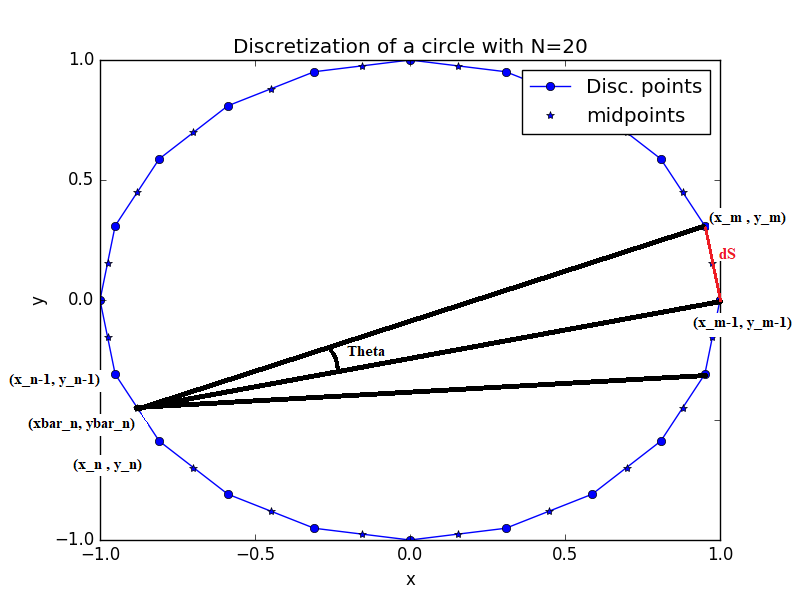
\includegraphics[width=7cm, height=5.5cm]{Discr_Circle.png} 
\caption{}
\label{fig:1a}
\end{subfigure}
\begin{subfigure}{0.4\textwidth}
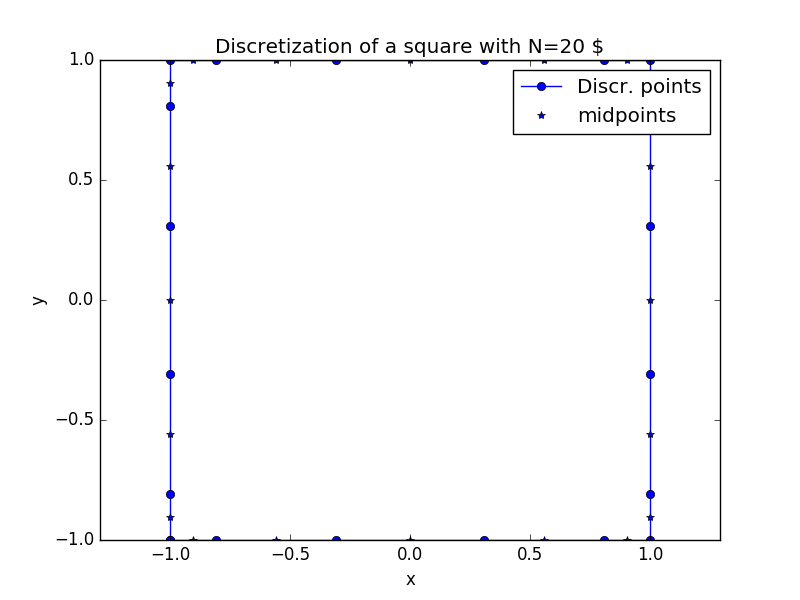
\includegraphics[width=5.5cm, height=5.5cm]{Discr_Square.png}
\caption{}
\label{fig:1b}
\end{subfigure}

\begin{subfigure}{0.4\textwidth}
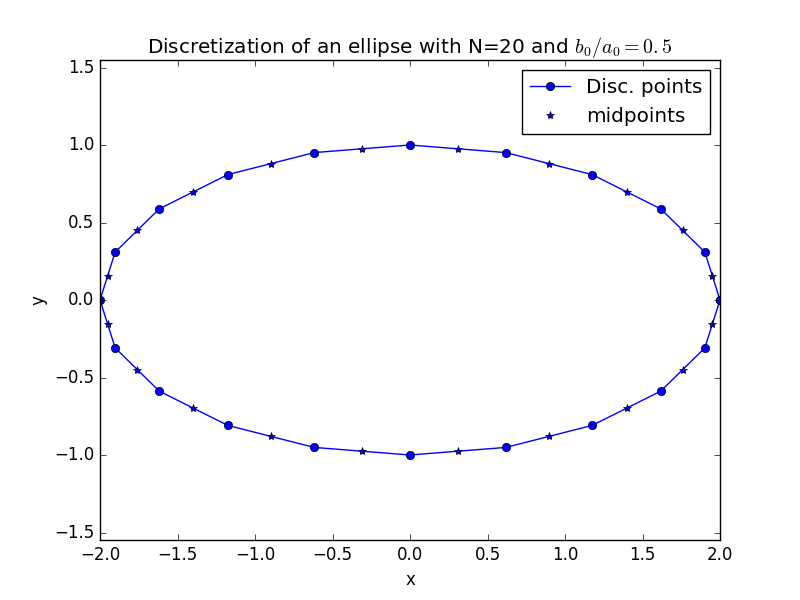
\includegraphics[width=5.5cm, height=5.5cm]{Discr_Ellipse_2_1.png} 
\caption{}
\label{fig:1c}
\end{subfigure}
\begin{subfigure}{0.4\textwidth}
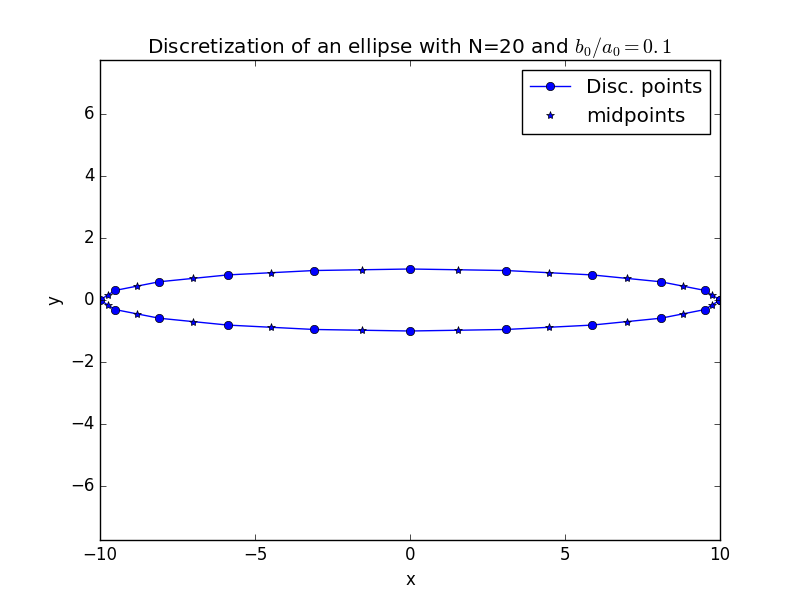
\includegraphics[width=5.5cm, height=5.5cm]{Discr_Ellipse_10_1.png}
\caption{}
\label{fig:1d}
\end{subfigure}

\caption{Discretization of surfaces with different shapes using $N=20$ segments. }
\label{fig:1}
\end{figure}

The $(x,y)$ points, shown by small circles on the surfaces in figure:(\ref{fig:1}), are then the end/start points of the segments. The discrete equation:(\ref{eq:1}) may be satisfied in the centroid of each segment at $(\bar{x}_i, \bar{y}_i) = (\frac{1}{2}(x_{i-1} + x_i),\frac{1}{2}(y_{i-1}+y_i))$. These points are marked with stars on figure:(\ref{fig:1}).\\

The length of each segment $dS$ is then  approximated by a straight line from a point on the surface to the next one. This length is then used to obtain an approximation for the unit normal vectors on the body surface, and as we can see from equation:(\ref{eq:2}) it will also be used to obtain an approximation for the integral $\int_{S_m} log r dS$.\\

For the unit normal vectors we have the following expressions:\\
\begin{equation*}
n_1 = -\frac{dy}{dS} \quad , \quad n_2 = \frac{dx}{dS} \quad , \quad n_6 = \textbf{r} \times \textbf{n} = x n_2 - y n_1
\end{equation*}
$\textbf{n}= (n_1, n_2)$ is the normal vector on segment $S_m$, pointing out of the fluid. The flux integral $\int_{S_m} (\frac{\dd}{\dd n}) log r dS$ equals the negative(since the normal is pointing into the geometry) of the opening angle $-\Delta \Theta_{n,m}$, defined by the segment $S_m$, such that equation:(\ref{eq:1}) can be expressed in the following discrete form: 

\begin{equation}\label{eq:3}
-\pi \phi_n + \sum_{m=1}^N \phi_m(\Delta \Theta_{n,m})=\sum_{m=1}^N \big[ \frac{\partial \phi}{\partial n} \big]_i h_{n,m, \quad n=1,2,...,N}
\end{equation}

Where $\frac{\dd \phi_i}{\dd n}$ equals $n_i$ on the surface $S$ and then equation:(\ref{eq:2}) is evaluated by the use of 2-point Gaussian quadrature rule. We can now solve equation:(\ref{eq:3}), by simply solving the equation $A \phi = B$, where A is a matrix of all the values for the opening angles on the left hand side of equation:(\ref{eq:3}). We can find these angles by using the law of cosines which is a generalization of the Pythagorean theorem. We will have $- \pi$ on the diagonal of the $A$ matrix. We can clearly see from figure:(\ref{fig:1a}) that when $n=m$ we have only a straight line and thus the angle must be equal to $\pi$. The right hand side of equation:(\ref{eq:3}) equals vector B.\\ 
Obtaining a solution for the potential $\phi$ will then help us with finding the added mass coefficients which are calculated by the following approximation:

\begin{equation}\label{eq:4}
m_{ji} = \rho \int_S \phi_j n_i dS \approx \rho \sum_{m=1}^N [\phi_j]_m [n_i]_m \Delta S_m
\end{equation}

For cases of flow around objects, we need to consider the additional effect resulting from the fluid acting on the object. These forces or effects represented by the added mass coefficients, can also arise in a direction due to motion in a different direction . Also the added mass depends not only on the geometry of the body but also on the direction of the acceleration. In a physical sense we can think of these added mass coefficients as a weight added to a motion system due to the fact that an accelerating or decelerating body moves some volume of the surrounding fluid with it as it moves, and the added mass force will then oppose the motion.\\[1em] 

When we look at a two dimensional body, we identify three degrees of freedom, since a degree of freedom represents the freedom to move in an independent way, then a two dimensional body can have a linear motion in the lateral and the longitudinal direction, but also a rotational motion. When we consider the added mass coefficients  $m_{ij}$ along such body, we can think of each component as the mass associated with a force on the object moving in the fluid in the $i^{th}$ direction due to a unit acceleration in the $j^{th}$ direction. When considering a two dimensional body the indexes \textit{i} and \textit{j} can have values 1, 2 and 6 and the added mass coefficients will then form a $3 \times 3$ matrix. Also the added mass is a pressure force per unit acceleration acting on a body, due to the acceleration field set up in the surrounding fluid. It is different in different degrees of motion and depends upon the  geometry of the body.\\[1em]

For symmetric geometries such as the geometries discussed in this assignment, the added mass tensor simplifies significantly. In the case of a circle as well as a square the lateral and longitudinal motion yields similar geometry and thus $m_{11} = m_{22}$, and also in the case of a circle the rotational added mass coefficient $m_{66}$  will be equal to zero.

\section*{Implementation for the case with a circle and an ellipse}
Following python script solves the discrete equations:(\ref{eq:3}) and (\ref{eq:4}) in the case for a circle and an ellipse. The results are then discussed and compared to the analytical solutions to the equations.

\begin{lstlisting}[language=Python]
from numpy import *
from matplotlib.pyplot import *
import warnings
warnings.filterwarnings('ignore')
import exceptions	

N_list = [100, 200, 400, 1000] # Number of segments								 

def Ellipse_Circle(a,b,N):
	"""
	Function for calculating the potential and added mass coefficients 
	for an ellipse where a is the major half axis and b is the minor 
	half axis. When a=b=R0 we have a circle.
	"""
	print

	if a==b:
		print('For a circle with radius R0 = %.2f' % a)
		print

	elif a>b:
		print('For an ellipse with major half axis a0 = %.2f' '\n'
				'and minor half axis b0 = %.2f' % (a, b))
		print

	else:
		raise exceptions.AssertionError('The major half axis a must be larger than the minor half axis b')
		# As required in the text for the assignment

	# Values for the potential and the added mass coefficients. achieved from 
	# different choice of N that needs to be stored in lists for later use
	phi11_ = []
	Exact_phi_ = []
	m11_ = []
	m22_ = []
	m66_ = []

	for N in N_list:
		print 'With %d segments we have:' % N

		# Matrix for storing values achieved from the lhs of the equation
		A = zeros((N,N))  

		# Array(vector) for storing values for the rhs of the equation 
		B11 = zeros(N)                                          
		B22 = zeros(N)											
		B66 = zeros(N)	

		dtheta = linspace(0, 2*pi, N+1) # division into N segments
		# Evaluation points
		x = a*cos(dtheta) # the x position of the start/end point of a segment
		y = b*sin(dtheta) # the y position of the start/end point of a segment

		# Collocation points
		# Centroid of each segment S(i)
		xbar = (x[1:] + x[:-1])/2.0
		ybar = (y[1:] + y[:-1])/2.0

		# Length of each segment dS = sqrt(d(x0,y0)^2 - d(x1,y1)^2)
		# (x,y) position - next (x,y) position
		dS = linalg.norm(array([x[1:],y[1:]])-array([x[:-1],y[:-1]]), axis=0) 

		# Normal vector components of the segments
		n1 = -(y[1:] - y[:-1])/dS 	# -dy/dS					       	 		 
		n2 = (x[1:] - x[:-1])/dS 	# dx/dS							               
		n6 = (xbar*n2 - ybar*n1)  	# x*n2 - y*n1

		for i in range(N):
			# Array transpose to get [x,y] position of a point on the body surface
			r1 = linalg.norm(array([x[:-1],y[:-1]]).T - array([xbar[i], ybar[i]]), axis=1)

			r2 = linalg.norm(array([x[1:],y[1:]]).T - array([xbar[i], ybar[i]]), axis=1)


			# Opening angle of segment S(i)
			theta = -arccos((dS**2 - r2**2 - r1**2)/(-2*r2*r1)) 
			theta[isnan(theta)] = 0	

			#Calculates the right-hand side of the integral eq.(24)
			h11 = (log(r1)+log(r2))*0.5*dS             
			h22 = (log(r1)+log(r2))*0.5*dS		     
			h66 = (log(r1)+log(r2))*0.5*dS

			#Adds the angles to the matrix A	    
			A[i] = theta # N matrices that are NxN
			fill_diagonal(A,-pi) #replace diagonal entries with -pi

			#Adds rhs to the B-arrays					    
			B11[i] = sum(n1*h11) 										 
			B22[i] = sum(n2*h22) 								 
			B66[i] = sum(n6*h66) 

		# Calculates phi for the three directions
		# Solve the linear matrix equation A*phi=B
		phi11 = linalg.solve(A,B11)
		phi11_.append(phi11)	
								 
		phi22 = linalg.solve(A,B22)								 
		phi66 = linalg.solve(A,B66)

		# Calculates the added mass coefficients
		m11 = sum(phi11*n1*dS)
		m11_.append(m11)
		
		m22 = sum(phi22*n2*dS)
		m22_.append(m22)

		m66 = sum(phi66*n6*dS)
		m66_.append(m66)	

		if a>b:
			Exact_m11 = pi*b**2
			Error_m11 = Exact_m11-m11
			print('The error in the added mass coefficient m11 is %.5f' % Error_m11)

			Exact_m22 = pi*a**2
			Error_m22 = Exact_m22-m22
			print('The error in the added mass coefficient m22 is %.5f' % Error_m22)

			Exact_m66 = (1.0/8.0)*pi*((a**2) - (b**2))**2
			Error_m66 = Exact_m66-m66
			print('The error in the added mass coefficient m66 is %.5f' % Error_m66)
			print

		if a==b:
			Exact_phi = -(a**2*xbar)/(xbar**2 + ybar**2)
			Exact_phi_.append(Exact_phi)
			Error_phi = abs(Exact_phi-phi11).max()
			print('The maximum error between the exact and the numerical potential is %.5f' % Error_phi)
			
			Exact_m11 = pi*a**2
			Error_m11 = Exact_m11-m11
			print('The maximum error between the exact and the numerical added mass coefficient m11 is %.5f' % Error_m11)
			print

	#return m11_, m22_, m66_, Exact_m11, Exact_m22, Exact_m66 	# in case of an ellipse
	return phi11_, Exact_phi_, m11_, Exact_m11 		# in case of a circle
            
\end{lstlisting}
\vspace{4mm}

The following code calls to the function Ellipse\_Circle to be solved for a circle with radius 1. The results are than compared to the analytical results.

\subsection*{Circle}
\begin{lstlisting}[language=Python]
#Circle

from Ellipse_function import *

colors = ['r', 'c', 'k', 'g', 'b']

phi11_, Exact_phi_, m11_, Exact_m11 = Ellipse_Circle(1, 1, N_list)

# Comparing analytical and numerical results for the potential
for i in range(len(N_list)):
	plot(phi11_[i], '-', color=colors[i], label='N=%d' % N_list[i])
	plot(Exact_phi_[i], '-', color=colors[i+1], label='Analytical solution')
	title('Analytical vs Numerical solution for the potential ' '$\phi_1$')
	xlabel('$Number$ $of$ $segments$ $N$', fontsize=18)
	ylabel('$\phi_1$', fontsize=24)
	legend(loc='upper right', numpoints = 1)
	savefig('Analytical_vs_numerical.png')
	show()

for i in range(len(N_list)):
	plot(1.0/N_list[i], m11_[i]/Exact_m11,'*', color=colors[i], markersize=16, linewidth=10, label='N=%d' %N_list[i])
	title('Computed added mass ' '$m_{11}$' ' divided by the analytical ' '$m_{11}$')
	hold(True)
	xlim((0, 0.011))
	ylabel('$m_{11}$' '/' ' Exact ' '$m_{11}$', fontsize=16)
	xlabel('1/N', fontsize=20)
	legend(loc='upper right', numpoints = 1)
show()

\end{lstlisting}

\subsection*{Results}
\begin{table}[H]
    \centering
    \begin{tabular}{|c|c|c|}\hline
    n  & Error in $\phi_1$       & Error in $m_{11}$  \\ \hline
    100 & 0.01452  & 0.04460   \\ \hline
    200 & 0.00710  & 0.02204   \\ \hline
    400 & 0.00351  &  0.01095  \\ \hline
    1000 & 0.00139 & 0.00437  \\ \hline
    \end{tabular}
    \caption{Error in the computed value for $\phi_1$ and the longitudinal added mass $m_{11}$ which equals the lateral added mass $m_{22}$ along a circle with radius 1 for different number of segments.}
    \label{tab:1}
\end{table}

\begin{figure}[H]
 \centering
\begin{subfigure}{0.4\textwidth}
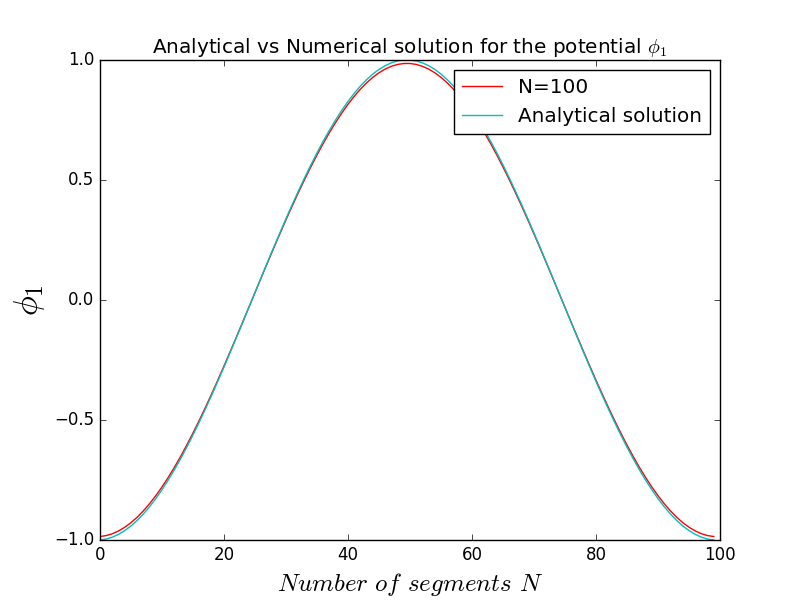
\includegraphics[width=6cm, height=6cm]{Circle1_potential_N100.png} 
\caption{$N=100$ }
\label{fig:2a}
\end{subfigure}
\begin{subfigure}{0.4\textwidth}
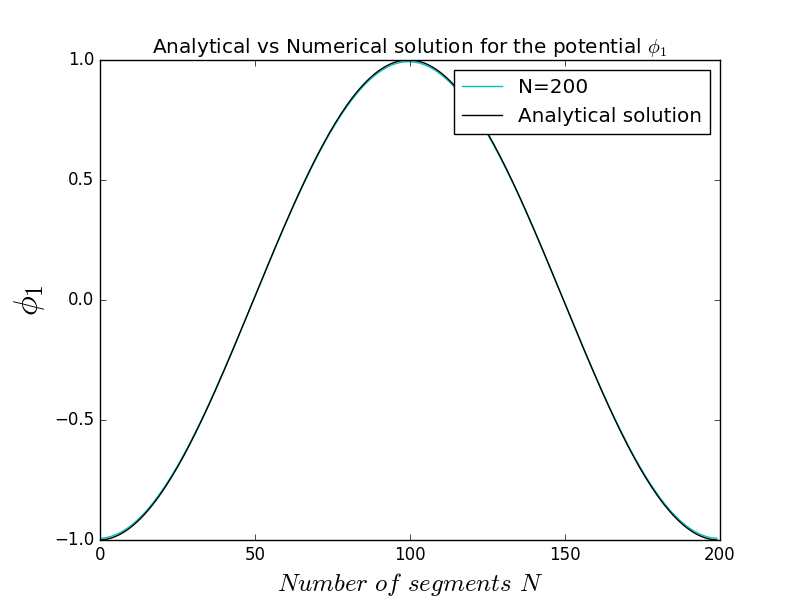
\includegraphics[width=6cm, height=6cm]{Circle1_potential_N200.png}
\caption{$N=200$ }
\label{fig:2b}
\end{subfigure}

\begin{subfigure}{0.4\textwidth}
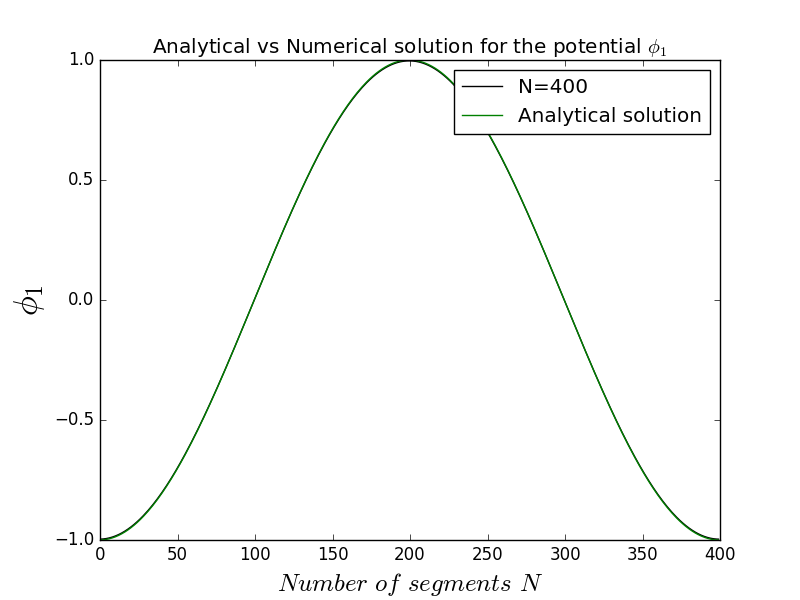
\includegraphics[width=6cm, height=6cm]{Circle1_potential_N400.png} 
\caption{$N=400$ }
\label{fig:2c}
\end{subfigure}
\begin{subfigure}{0.4\textwidth}
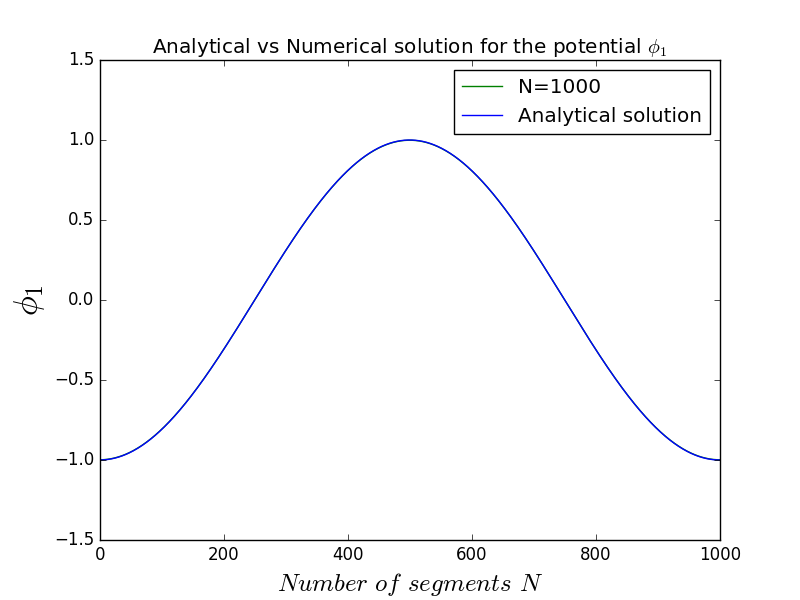
\includegraphics[width=6cm, height=6cm]{Circle1_potential_N1000.png}
\caption{$N=1000$ }
\label{fig:2d}
\end{subfigure}
 
\caption{Numerically computed potential $\phi_1$ along a circle compared to the analytical $\phi_1 = -\frac{R_0^2 x}{x^2 + y^2}$ as function of number of segments.}
\label{fig:2}
\end{figure}

As we can see from table:(\ref{tab:1}), the error is very small even with small number of segments and it goes towards zero as N increases. \\
Figure:(\ref{fig:2}) shows that as the resolution improves, we will have convergence of the numerical solution for $\phi_1$ to the analytical solution for the potential for a circle with radius $R_0$ performing a translation in the x or y-direction. For $N=1000$ the two graphs coincide completely. \\


\begin{figure}[H]
  \begin{center}
    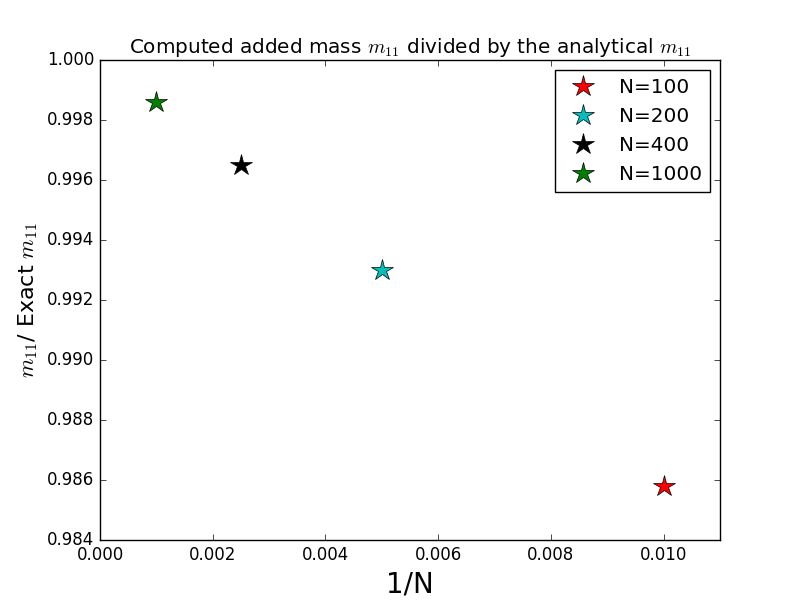
\includegraphics[width=6cm, height=6cm]{Circle1_m11_conv.png}
  \end{center}
  \caption{Computed added mass $m_{11}$ of the circle divided by the analytical added mass $\rho \pi R_0^2$ as a function of the inverse of the resolution.}
  \label{fig:3}
\end{figure}

Figure:(\ref{fig:3}) shows also convergence of the computed values for $m_{11}=m_{22}$ to the analytical one, which corresponds to the displaced mass of the area of the circle, as we get a better resolution in the discretization of the circle. 

\subsection*{Ellipse}
The following code calls to the function Ellipse\_Circle to be solved for an ellipse, first with $a_0 = 2$ and $b_0 = 1$ such that $\frac{b_0}{a_0} = 0.5$ and then with $a_0 = 10$ and $b_0 = 1$ such that $\frac{b_0}{a_0} = 0.1$. The numerical results are than compared to the analytical results.\\[2em]
\begin{lstlisting}[language=Python]
#Ellipse

from Ellipse_function import *


colors = ['r', 'g', 'k', 'c']

#m11_, m22_, m66_, Exact_m11, Exact_m22, Exact_m66 = Ellipse_Circle(2, 1, N_list)

m11_, m22_, m66_, Exact_m11, Exact_m22, Exact_m66 = Ellipse_Circle(10, 1, N_list)


#checking for convergence
for i in range(len(N_list)):
	plot(1.0/N_list[i], m11_[i]/Exact_m11,'*', color=colors[i], markersize=14, label='$m_{11}$')
	hold(True)
	plot(1.0/N_list[i], m22_[i]/Exact_m22,'s', color=colors[i], markersize=14, label='$m_{22}$')
	hold(True)
	plot(1.0/N_list[i], m66_[i]/Exact_m66,'^', color=colors[i], markersize=14, label='$m_{66}$')

	if i==0:
		legend(loc='best', numpoints = 1)

title('Convergence for the computed added mass coefficients ' '$m_{11}$' ', $m_{22}$' ' and ' '$m_{66}$')
hold(True)
xlim((0, 0.011))
ylim((0.91 , 1.005))
ylabel('Numerical added mass coefficients/Exact values', fontsize=14)
xlabel('  1/N , (same colors show the same number of segments)', fontsize=14)
show()

\end{lstlisting}

\newpage 

The analytical results for the added mass coefficients along an ellipse are as follows:
\begin{align*}
m_{11} = \rho \pi b_0^2 \quad , \quad m_{22} = \rho \pi a_0^2 \quad , \quad m_{66} = \frac{1}{8} \rho \pi (a_0^2 - b_0^2)^2
\end{align*}

These exact values for the added mass coefficients are used to investigate the convergence for the computed values in figure:(\ref{fig:4}).

\begin{figure}[H]
 \centering
 
\begin{subfigure}{0.4\textwidth}
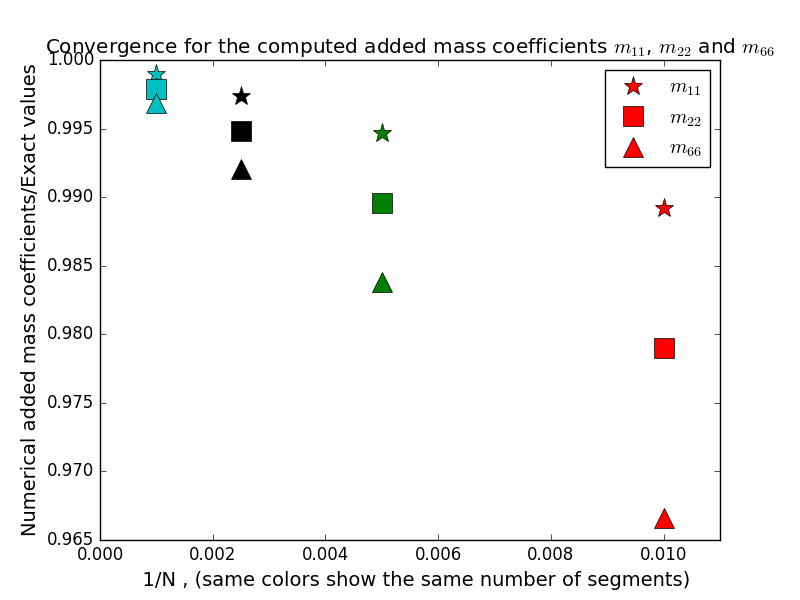
\includegraphics[width=7cm, height=7cm]{Ellipse_2_1_conv.png} 
\caption{Convergence of the added mass coefficients along an ellpise where $\frac{b_0}{a_0}=0.5$ }
\label{fig:4a}
\end{subfigure}
\begin{subfigure}{0.4\textwidth}
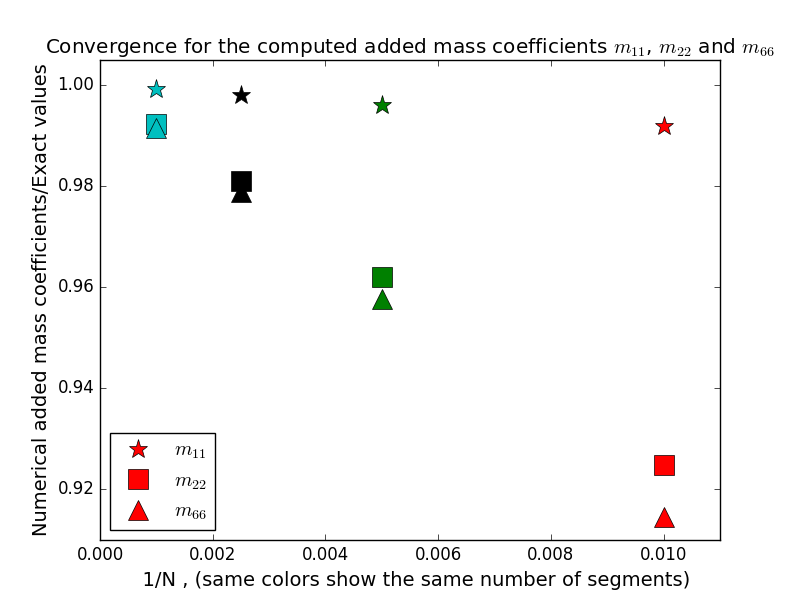
\includegraphics[width=7cm, height=7cm]{Ellipse_10_1_conv.png}
\caption{Convergence of the added mass coefficients along an ellpise where $\frac{b_0}{a_0}=0.1$}
\label{fig:4b}
\end{subfigure}
 
\caption{Numerically computed added mass coefficients divided by the analytical ones along an ellipse as a function of the inverse of the resolution.}
\label{fig:4}
\end{figure}
 
Figure:(\ref{fig:4}) show the ratio of the computed added mass coefficients divided by the corresponding analytical ones. We can see that this ratio converges towards 1 as $\frac{1}{N}$ tends to zero, but as we can see we get good convergence in $m_{11}$ and $m_{22}$ even with small numbers for $N$, so the convergence occurs much faster than for $m_{66}$ and as we can see, we get the best approximation when we have motion in the x-direction. Therefore I think it would be a good idea to investigate the error between the exact and the numerical solutions more closely. Specially in the case where $\frac{b_0}{a_0} = 0.1$.

\begin{table}[H]
    \centering
    \caption{The Error in the numerical solution for the added mass coefficients for an ellipse with $\frac{b_0}{a_0}=0.5$ on the top and with $\frac{b_0}{a_0}=0.1$ at the bottom.}
    \label{tab:2}
    \begin{tabular}{|c c|c|c|c|}
        \toprule
      &$\frac{b_0}{a_0}=0.5 \vert$ N  & Error in $m_{11}$ & Error in $m_{22}$ & Error in $m_{66}$  \\
        \midrule
      &  100  &  0.03396 &  0.26348 & 0.11808 \\ \hline
      &  200 &  0.01666 &  0.13118 & 0.05710 \\ \hline
      &  400 &  0.00825 &  0.06546 & 0.02806 \\ \hline
      &  1000 &  0.00328 &  0.02615 & 0.01110 \\ \hline
    \end{tabular}
    \begin{tabular}{|c c|c|c|c|}
     &$\frac{b_0}{a_0}=0.1 \vert$ N  & Error in $m_{11}$ & Error in $m_{22}$ & Error in $m_{66}$  \\
        \midrule
      &  100  &  0.02544 &  23.62821 & 328.78271 \\ \hline
      &  200 &  0.01235 &  11.89113 & 162.94352 \\ \hline
      &  400 &  0.00608 &  5.96638 & 81.09127 \\ \hline
      &  1000 &  0.00241 &  2.39177 & 32.34333 \\ \hline
    \end{tabular}\vspace{1cm}
\end{table}
As we can see from table:(\ref{tab:2}), the difference between the exact and the numerical value for the rotational added mass $m_{66}$ for an ellipse with the major half axis ten times longer than the minor half axis, is a bit too large, even though it will also converge towards the exact solution as N increases.\\[1em]

For a closer investigation of the error for the added mass coefficients along an ellipse where $\frac{b_0}{a_0}=0.1$, I made a plot of the error for the longitudinal, lateral and rotational added mass coefficients (figure:(\ref{fig:5})). It seems that for small values for $N$ the numerical value for $m_{66}$ is much smaller than the exact one and by doubling the number of $N$ values, we get half the error.  It seems that this error is directly related to the discretization of the body and the fact that the rotational and the lateral added mass along an ellipse with the major half axis 10 times larger than the minor half axis have larger values compared to the longitudinal one, but I was not able to figure out a good fix to this error issue.

\begin{figure}[H]
    \centering
    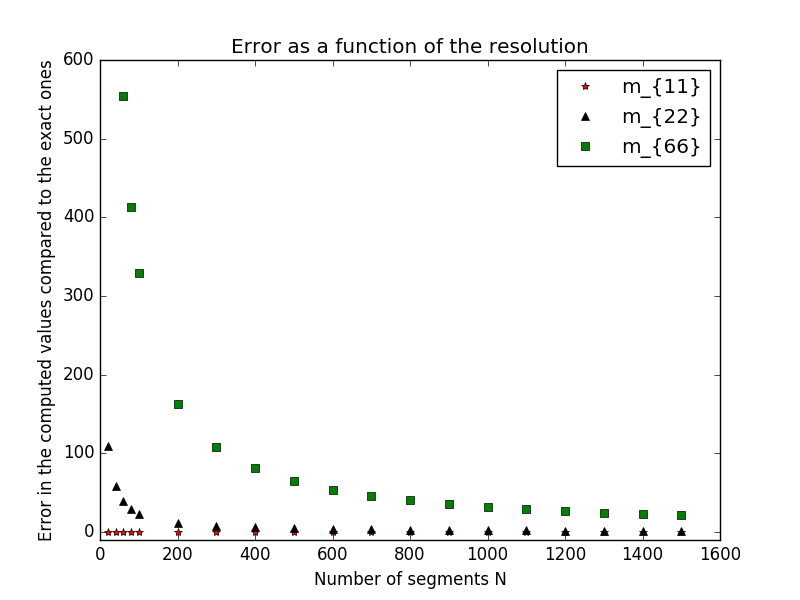
\includegraphics[width=10cm, height=10cm]{Error10.png} 
    \caption{Error in added mass components as a function of the resolution for an ellipse with major half axis $a_0 = 1.0$ and minor half axis $b_0 = 10$}
    \label{fig:5}
\end{figure}

\section*{Implementation for the case with a square}
The exact longitudinal, lateral and rotational added mass coefficients along a square are:

\begin{equation*}
m_{11} = m_{22} = 4.754 \rho a_0^2 \quad , \quad m_{66} = 0.725 \rho a_0^4
\end{equation*}

Following python code solves equation (\ref{eq:1}) and (\ref{eq:3}) for the potential and the added mass coefficients along a square with side lenghts of $2a_0$.

\begin{lstlisting}[language=Python]
from numpy import *
from matplotlib.pyplot import *
import warnings
warnings.filterwarnings('ignore')

N_list=[100, 200, 400, 1000] # Number of segments
def square(a, N):
	"""
	Function for calculating the potential and added 
	mass of coefficients for a square.
	"""
	print('For a square with side length of 2a = %.2f' % (2*a))
	
	m11_ = []
	m22_ = []
	m66_ = []

	for N in N_list:
		print 'With %d segments we have:' % N
		# Matrix for storing values achieved from the lhs of the equation
		A = zeros((N,N))  

		# Array(vector) on the rhs os the equation 
		B11 = zeros(N)                                          
		B22 = zeros(N)											
		B66 = zeros(N)

		x = zeros(N+1)
		y = zeros(N+1)

		S1 = -a # Negative half of a side
		S2 = a  # Positive half of the side

		N = N/4 * 4 	# Total number of segments for all the four sides										 
		N1 = N/4 
				# Number of segments for one side										 
		x = zeros(N+1)
		y = zeros(N+1)

		#making points in all four sides
		for i in range(N1+1):
			inc = a*(1-(cos(pi/N1*i))) # from a to 2a

			# Bottom side (Constant y=-a while x goes from -a to a)
			x[i] = S1 + inc
			y[i] = -a

			# Right side (Constant x=a while y goes from -a to a)
			x[i+N1] = a
			y[i+N1] = S1 + inc

			# Top side (Constant y=a while x goes from a to -a)
			x[i+2*N1] = -(S1 + inc)
			y[i+2*N1] = a

			# Left side (Constant x=-a while y goes from a to -a)
			x[i+3*N1] = -a
			y[i+3*N1] = -(S1 + inc)

		# midpoint values for x and y (center of each segment)
		xbar = (x[1:] + x[:-1])/2.0
		ybar = (y[1:] + y[:-1])/2.0
		

		# Length of each segment dS = sqrt(d(x0,y0)^2 - d(x1,y1)^2)
		# (x,y) position minus the next (x,y) position
		dS = linalg.norm(array([x[1:],y[1:]])-array([x[:-1],y[:-1]]), axis=0) 

		# Normal vector components of the segments
		n1 = -(y[1:] - y[:-1])/dS 	#-dy/dS					       	 		 
		n2 = (x[1:] - x[:-1])/dS 	#dx/dS							               
		n6 = (xbar*n2 - ybar*n1) 

		for i in range(N):
			# array transpose to get [x,y] position of a point on the body surface
			# Distance from midpoint in segment i to the starting/ending point of the
			# next/current segment
			r1 = linalg.norm(array([x[:-1],y[:-1]]).T - array([xbar[i], ybar[i]]), axis=1)

			r2 = linalg.norm(array([x[1:],y[1:]]).T - array([xbar[i], ybar[i]]), axis=1)

			theta = -arccos((dS**2 - r2**2 - r1**2)/(-2*r2*r1)) 
			theta[isnan(theta)] = 0	

			#Calculates the right-hand side of the integral (24)
			h11 = (log(r1)+log(r2))*0.5*dS             
			h22 = (log(r1)+log(r2))*0.5*dS		     
			h66 = (log(r1)+log(r2))*0.5*dS

			#Adds the angles to the matrix A	    
			A[i] = theta # N matrices that are NxN
			fill_diagonal(A,-pi) #replace diagonal entries with -pi

			#Adds rhs to the B-arrays					    
			B11[i] = sum(n1*h11) 										 
			B22[i] = sum(n2*h22) 								 
			B66[i] = sum(n6*h66) 

		# Calculates phi for the three directions
		# Solve the linear matrix equation A*phi=B
		phi11 = linalg.solve(A,B11)							 
		phi22 = linalg.solve(A,B22)								 
		phi66 = linalg.solve(A,B66)

		# Calculates the added mass coefficients
		m11 = sum(phi11*n1*dS)
		m11_.append(m11)

		m22 = sum(phi22*n2*dS)
		m22_.append(m22)

		m66 = sum(phi66*n6*dS)
		m66_.append(m66)	

		Exact_m11 = 4.754*a**2
		Error_m11 = Exact_m11-m11
		print('The error in the added mass coefficient m11 is %.5f' % Error_m11)

		Exact_m22 = 4.754*a**2
		Error_m22 = Exact_m22-m22
		print('The error in the added mass coefficient m22 is %.5f' % Error_m22)

		Exact_m66 = 0.725*a**4
		Error_m66 = Exact_m66-m66
		print('The error in the added mass coefficient m66 is %.5f' % Error_m66)
		print

	return m11_, Exact_m11, m22_, Exact_m22, m66_, Exact_m66
\end{lstlisting}

The following script calls to the function square with a sidelength of $2a$. The results are than compared to the analytical results.

\begin{lstlisting}[language=Python]
#Square

from square_function import *

colors = ['r', 'c', 'k', 'g', 'b']

m11_, Exact_m11, m22_, Exact_m22, m66_, Exact_m66 = square(1, N_list)

#checking for convergence
for i in range(len(N_list)):
	plot(1.0/N_list[i], m11_[i]/Exact_m11,'*', color=colors[i], markersize=14, label='$m_{11} = m_{22}$')
	hold(True)
	plot(1.0/N_list[i], m66_[i]/Exact_m66,'^', color=colors[i], markersize=14, label='$m_{66}$')

	if i==0:
		legend(loc='best', numpoints = 1)

title('Convergence for the computed added mass coefficients ' '$m_{11}$' ', $m_{22}$' ' and ' '$m_{66}$')
hold(True)
xlim((0, 0.011))
ylim((0.90 , 1.005))
ylabel('Numerical added mass coefficients/Exact values', fontsize=14)
xlabel('  1/N , (same colors show the same number of segments)', fontsize=14)
show()
"""
#output

With 100 segments we have:
The error in the added mass coefficient m11 is 0.11908
The error in the added mass coefficient m22 is 0.11908
The error in the added mass coefficient m66 is 0.06435

With 200 segments we have:
The error in the added mass coefficient m11 is 0.06120
The error in the added mass coefficient m22 is 0.06120
The error in the added mass coefficient m66 is 0.03207

With 400 segments we have:
The error in the added mass coefficient m11 is 0.03116
The error in the added mass coefficient m22 is 0.03116
The error in the added mass coefficient m66 is 0.01620

With 1000 segments we have:
The error in the added mass coefficient m11 is 0.01272
The error in the added mass coefficient m22 is 0.01272
The error in the added mass coefficient m66 is 0.00673
"""
\end{lstlisting}

\subsection*{Results}

\begin{table}[H]
    \centering
    \begin{tabular}{|c|c|c|c|}\hline
    N  & Error in $m_{11} = m_{22}$  & Error in $m_{66}$   \\ \hline
    100 & 0.11908  & 0.06435  \\ \hline
    200 & 0.06120  & 0.03207   \\ \hline
    400 & 0.03116  & 0.01620  \\ \hline
    1000 & 0.01272 & 0.00673   \\ \hline
    \end{tabular}
    \caption{The Error in the numerical approximation for the added mass coefficients along a square with side length of $2 a_0$}
    \label{tab:3}
\end{table}

As we can see from the output of the code used to compute the potential and the added mass coefficients, the lateral and the longitudinal added masses are equal as expected.\\[1em]

\begin{figure}[H]
 \centering
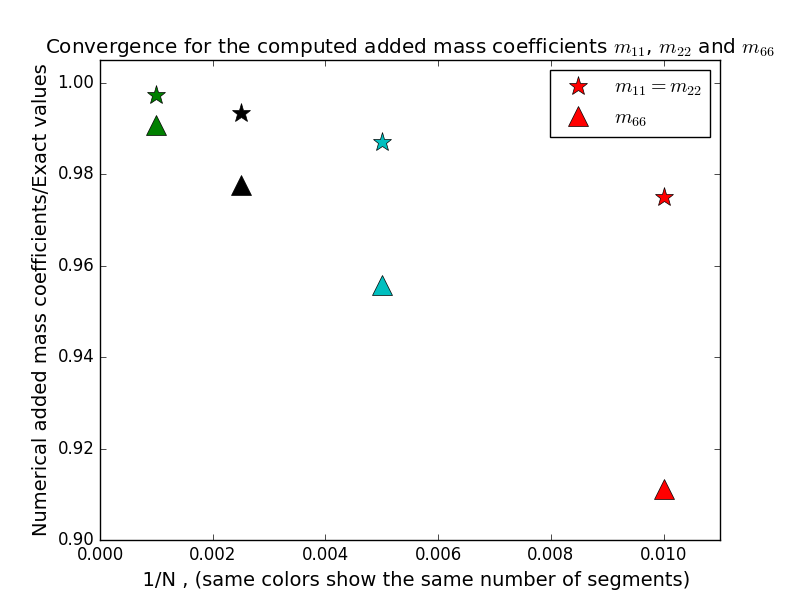
\includegraphics[width=9cm, height=8cm]{square1_conv.png} 
\caption{Numerically computed added mass coefficients divided by the analytical ones along a square with side length of $2 a_0 = 2$ as a function of the inverse of the resolution.}
\label{fig:6}
\end{figure}

Figure:(\ref{fig:6}) shows convergence of the computed values for $m_{11}$ and $m_{66}$ as the resolution improves, also as $\frac{1}{N}$ tends to zero. We can also see the convergence from table:(\ref{tab:3}), where we can see that the error between the exact and the approximated values for the added masses decrease as N increases.\\

\end{document}